\documentclass{article}

% if you need to pass options to natbib, use, e.g.:
% \PassOptionsToPackage{numbers, compress}{natbib}
% before loading nips_2017
%
% to avoid loading the natbib package, add option nonatbib:

\PassOptionsToPackage{numbers, compress}{natbib}
\usepackage[final]{nips_2017}

% to compㅁle a camera-ready version, add the [final] option, e.g.:
\usepackage[utf8]{inputenc} % allow utf-8 input
\usepackage[T1]{fontenc}    % use 8-bit T1 fonts
\usepackage{hyperref}       % hyperlinks
\usepackage{url}            % simple URL typesetting
\usepackage{booktabs}       % professional-quality tables
\usepackage{amsfonts}       % blackboard math symbols
\usepackage{nicefrac}       % compact symbols for 1/2, etc.
\usepackage{microtype}      % microtypography
\usepackage{amsmath, amssymb, amsfonts, amsthm}
\usepackage[export]{adjustbox}
\usepackage{subcaption}
\usepackage[font=small]{caption}
\usepackage{todonotes}
%\usepackage[]{algorithm2e}
\usepackage{algorithm}
\usepackage[noend]{algpseudocode}
\usepackage{booktabs}

% Some reference styles
\newcommand{\eref}[1]{(\ref{#1})}% Equation
\newcommand{\aref}[1]{Algorithm~\ref{#1}}% Algorithm
\newcommand{\sref}[1]{Section~\ref{#1}}% Section
\newcommand{\figref}[1]{Figure~\ref{#1}}% Figure
\newcommand{\tabref}[1]{Table~\ref{#1}}% Table

\DeclareMathOperator*{\argmax}{arg\,max}
\DeclareMathOperator*{\argmin}{arg\,min}
\bibliographystyle{ieeetr}

\title{Bayesian-Adaptive Deep Reinforcement Learning using Model Ensembles}

% The \author macro works with any number of authors. There are two
% commands used to separate the names and addresses of multiple
% authors: \And and \AND.
%
% Using \And between authors leaves it to LaTeX to determine where to
% break the lines. Using \AND forces a line break at that point. So,
% if LaTeX puts 3 of 4 authors names on the first line, and the last
% on the second line, try using \AND instead of \And before the third
% author name.

\author{
  Gilwoo Lee \\ \texttt{gilwoo@cs.uw.edu} \\
  \And
  Jeongseok Lee \\ \texttt{jslee02@cs.uw.edu} \\
  \And
  Brian Hou \\ \texttt{bhou@cs.uw.edu} \\
  \And
  Aditya Mandalika \\ \texttt{adityavk@cs.uw.edu} \\
}

\begin{document}

\maketitle

% \begin{abstract}
% lalala abstract!
% \end{abstract}

\section{Introduction}
Although model-free deep reinforcement learning algorithms have shown tremendous success in a wide range of tasks, such as simulated control problems in OpenAI Gym~\cite{openai-gym} and games like Go~\cite{alphago}, they face fundamental challenges in their application to physical control problems on robotic hardware.
The high sample complexity of current methods results in long training periods if applied directly to hardware, even for simple grasping tasks~\cite{levine2016armfarm}.
Furthermore, the safety of the robot or surrounding environment when gathering data from the real world may be difficult to guarantee while the policy is training.

Model-based reinforcement learning techniques offer an opportunity to overcome these issues by taking advantage of simulations of the real systems, which can generate training data faster than real time.
The primary challenge with model-based techniques is the discrepancy between simulation and the real world.
Simplified models, inaccurate or uncertain parameters that govern the dynamics of the model, and other unmodeled disturbances and noise can render the policies learned on the simulated model ineffective on the real system.

We propose a model-based algorithm that learns a universal policy for Bayes-Adaptive Markov Decision Process (BAMDP) that is robust and optimal to model uncertainty and disturbances. Although the real system's exact physical parameters are unknown, we can maintain a belief distribution over those parameters and provide this belief as an additional input to the policy.
This enables the learned policy to be bold when confident in its model and cautious when there is high model uncertainty.

\section{Related Work}
Our work is closely related to QMDP~\cite{littman1995learning, karkus2017qmdp} which is a Q-value approximation method for Partially Observable Markov Decision Processes (POMDPs).
QMDP assumes a fully-observable MDP after one action by approximating the Q-value at the current belief state $b(s)$ as a weighted average over the fully-observable MDP's Q-values, $Q_{\text{MDP}}(b, a) = \sum_s b(s)Q(s, a)$.
The algorithm requires access to the (approximate) Q-function for the MDP.
QMDP performs surprisingly well for many problems, but determinizing the belief distribution after one timestep breaks Bayes-optimality.


%In our problem setup, we have a belief over the physics parameters $\phi$ of the MDP, $b(\phi)$, and we compute the policy $Q_a(s;b) = \sum_\phi b(\phi)Q_{\text{MDP}}(s,a;\phi)$.
%
The BAMDP formulation that we consider is also similar to the POMDP formulation used in POMDP-lite~\cite{chen2016pomdp}, which assumes that the hidden state variables remain constant or only change deterministically.
In our case, the hidden state variables correspond to the physics parameters $\phi$.
Chen et al. show that this formulation is ``equivalent to a set of fully observable Markov decision processes indexed by a hidden parameter'', which, in our case, is a discretization of $\phi$.

Robustness to model uncertainty has also been addressed by EPOpt~\cite{rajeswaran2016epopt}, which learns a policy that maximizes the worst-case performance across multiple sampled MDPs.
However, as is common with min-max techniques, EPOpt can be quite conservative (and therefore far from optimal) in its policy, especially when the model's possible parameter-space is large.
Our work closes this gap in EPOpt by maintaining a belief over the training MDPs to balance between optimality and robustness.

Another recent approach to model uncertainty is UP-OSI~\cite{yu2017uposi}, which utilizes online system identification to estimate the physical parameters of the system.
However, UP-OSI only uses the mean estimate of those parameters as an additional input to the policy.
Without a notion of belief and uncertainty in its parameter estimates, UP-OSI is prone to aggressively executing policies without being conservative toward remaining model uncertainty.

% TODO: mention \cite{guez2014bayes} and other bayesian work.

\section{Bayes-Adaptive Reinforcement Learning}

\begin{figure*}[t!]
\centering
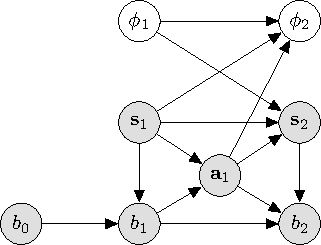
\includegraphics[width=0.5\linewidth]{figs/model.pdf}
\caption{Graphical model for a Bayes-Adaptive Markov Decision Process.}
\label{fig:pgm}
\end{figure*}

We follow the BAMDP framework (\figref{fig:pgm}), which assumes that a latent variable $\phi$ governs the transition function of the underlying Markov Decision Process~\cite{ghavamzadeh2015bayesian, ross2008bayes, guez2012efficient}.
A BAMDP is defined by a tuple $\langle \mathcal{S}', \mathcal{A}, P, P_0, R \rangle$, where
\begin{itemize}
\item $\mathcal{S'} = \mathcal{S}\times \Phi$ is the set of hyper-states (state $s$, latent variable $\phi$),
\item $\mathcal{A}$ is the set of actions,
\item $P(s',\phi'|s, \phi, a)$ is the transition function between hyper-states, conditioned
on action $a$ being taken in hyper-state $(s, \phi)$,
\item $P_0\in \mathcal{P}(\mathcal{S} \times \Phi)$ combines the initial distribution over hyper-states,
\item $R(s, \phi, a)$ represents the reward obtained when action $a$ is
taken in hyper-state $(s,\phi)$.
\end{itemize}
In our setting of robot control, the latent variables $\phi$ are physics parameters such as mass and length of different robot links.
% (TODO: better word than links) (JS: robot bodies?).

Our goal is to find the Bayes-optimal policy for the following Bellman equaton:
\begin{equation}\label{eq:rl}
V^*(b, s) = \max_a \bigg\{R(s, b, a) + \gamma \sum_{s'}P(s', b'|s, b, a)V^*(b', s') \bigg\}
\end{equation}
where $b(\phi)$ is the belief over the set of latent physics parameters $\phi \in \Phi$,
\begin{align*}
R(s, b, a)
  &= \sum_{\phi \in \Phi} b(\phi) R(s, \phi, a) \\
P(s', b' | s, b, a)
  &= \sum_{\phi \in \Phi} b(\phi) P(s', b' | s, \phi, a) \\
  &= \sum_{\phi \in \Phi} b(\phi) P(s' | s, \phi, a) \sum_{\phi' \in \Phi} P(\phi' | s, \phi, a).
\end{align*}

% TODO(?): mention PAC-MDP?

\subsection{Belief Update}

We make a simplification to the BAMDP formulation by assuming that the latent variable $\phi$ is constant or changing deterministically according to a known transition function.
% \footnote{
% A looser assumption is that the rate of change of $\phi$ is slow enough that approximating the long-term value with the same $\phi$ is a reasonable short-term approximation for choosing the one-step action, i.e. we can treat $V^*(s_t, \phi_t) \approx V^*(s_t, \phi_{t:\infty})$ for a one-step Bellman update.
% }
As in POMDP-lite\cite{chen2016pomdp}, we can then view the simplified BAMDP model as a set of MDPs that are indexed by the latent variable $\phi$.

% \begin{align*}
% b(\phi_t) = P(\phi_t|s_{t-1}, \phi_{t-1}, a_{t-1})
% \end{align*}
% which is then used to compute the best policy from an ensemble of $\phi$-dependent optimal policies, i.e., $\pi^*(\cdot;\phi)$ and $V^*(\cdot;\phi)$ are computed with typical RL algorithms for MDPs.
% Then the remaining task is to compute the one-step best action $a$:
% \begin{align}\label{eq:barl}
%  a^* &= \argmax_{a} \mathbb{E}_{\phi \sim b(\phi)} \bigg[R(s, a, \phi) + \gamma \sum_{s', \phi'}P(s',\phi'|s, \phi, a)V^{*'}(s', \phi') \bigg].
% \end{align}

The posterior probability of an MDP governed by latent physics variable $\phi$ given a trajectory $\tau_{0:H} = (s_0, a_0, \cdots, s_H)$ is given by:
\begin{align}
P(\phi_H | \tau_{0:H})
  &= \frac{1}{Z} P(\phi_0) P(\tau_{0:H} | \phi_0) \nonumber \\
  &= \frac{1}{Z} P(\phi_0) \prod_{t=0}^{H-1} P(s_{t+1}, \phi_{t+1} | s_t, \phi_t, a_t) \nonumber \\
  &= \frac{1}{Z} P(\phi_0) \prod_{t=0}^{H-1} P(s_{t+1}|s_t, \phi_t, a_t) P(\phi_{t+1} | s_t, \phi_t, a_t)
\end{align}
where $Z$ is a normalizing constant and $P(\phi_{t+1} | \cdot) = 1$ is the deterministic transition of $\phi$.

% Assuming that $\phi$ is constant allows us to simplify the belief update rule at each timestep $t$:
% \begin{align*}
% b_t(\phi) \propto \sum_{\phi \in \Phi} P(\phi|s_{t-1}, a_{t-1}) b_{t-1}(\phi)
% \end{align*}
% Our algorithm uses the state augmented with this updating belief as the input to the policy at each timestep.

\section{Bayes-Adaptive Policy Gradient}

\begin{figure*}[t!]
\centering
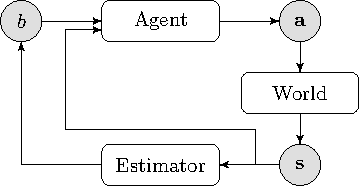
\includegraphics[width=0.5\linewidth]{figs/system_structure.pdf}
\caption{System structure}
\end{figure*}

The main contribution of our work is a policy-gradient algorithm which produces a universal policy that maintains different strategies for different beliefs. The key idea is to augment the state with the belief and provide this augmented feature as input to the policy. The policy is a function of both state and belief: $\pi: \mathcal{S} \times \mathcal{B} \rightarrow P(\mathcal{A})$, where $\mathcal{B}$ is the belief space. This allows the policy to differentiate between the beliefs while sharing globally effective strategies.

In order for this algorithm to work in practice, we need an effective representation of the belief space. If the space of MDPs $\mathcal{M}$ is finite, the belief $b$ can be a vector of size $|\mathcal{M}|$. If $\mathcal{M}$ is infinite, we propose two methods to approximate the belief space:

\begin{itemize}
    \item Sample $K$ MDPs from the prior belief distribution $b_0$ and use belief over these $K$ MDPs
    \item Discretize the parameter space and use belief over the parameter space
\end{itemize}
In the first case, we use a vector of size $K$ as $b$; $K$ should be large enough to approximate all MDPs with the $K$ sampled ones. In the second case, assuming the latent parameters are independent, the belief is represented as a vector of size $(N_1 + \cdots + N_M)$ where $M$ is the total number of parameters and $N_m$ is the discretization of the $m$-th parameter. In this project, we have implemented the first one, and leave the second one for future work.

The algorithm is shown in \aref{algo:bapg}. At each iteration, we sample a number of MDPs from the prior distribution $b_0$, and sample a trajectory for each MDP using the current policy. During the rollout of the trajectory, the estimator provides the updated belief estimate as an additional feature to the policy. The estimator resets to $b_0$ at the beginning of each trajectory.

Note that the policy observes the \emph{evolution} of belief along each trajectory. This allows the policy to learn to be optimal with respect to the evolution of belief, and to take actions which affect the evolution. For example, given prior belief $b_0$ with high entropy (i.e., high uncertainty), our algorithm policy would produce conservative or informative actions until $b$ becomes informative enough along the course of the trajectory. This is a key difference between our algorithm and UP-OSI~\cite{yu2017uposi}, in which the universal policy has no notion of belief or uncertainty.

%%\newcommand{\argmin}{\operatornamewithlimits{\arg\min}}
%
%
%------------------------------------------
% Algorithm:
%------------------------------------------%
\begin{algorithm}[tb]
\caption{Bayes-Adaptive Policy Gradient}
\label{algo:bapg}
\begin{algorithmic}[1]
\Require Bayes-Estimator $ES$, $b_0$, $\mathcal{M}$, initial policy $\theta_0$, $n_\text{itr}, n_\text{sample}$
\vspace{2mm}
\For{$i = 1, 2, \cdots, n_\text{itr}$}
  \For{$n = 1, 2 , \cdots, n_\text{sample}$}
    \State Reset $ES$ with $b_0$
    \State Sample model parameter $\phi \sim b_0$ to get $M_{\phi}$
    \State Sample a trajectory $\tau_n$ from $M_{\phi}$ using policy $\pi(\theta_i)$ and estimator $ES$
  \EndFor
  \State Update policy: $\theta_{i+1} = \texttt{BatchPolicyOptimization}(\theta_i, \{\tau_1, \cdots, \tau_{n_{sample}}\})$
\EndFor
\end{algorithmic}
\end{algorithm}

\section{Experiments}

Our algorithm falls under the class of model-based algorithms that consider multiple MDPs to train a policy.
We compare our algorithm against others from this class, QMDP~\cite{littman1995learning, karkus2017qmdp} and EPOpt~\cite{rajeswaran2016epopt}.
QMDP assumes that the latent state $\phi$ is revealed after one step, taking the action that maximizes $Q_{\text{MDP}}(s, a, b(\phi)) = \sum_{\phi \in \Phi} b(\phi) Q(s, a, \phi)$.
EPOpt is a minimax-style algorithm which trains the policy to be robust across multiple MDPs, without utilizing the belief over MDPs in learning the policy.

We evaluate the three algorithms on a set of simulated benchmark examples from OpenAI Gym~\cite{openai-gym} using the MuJoCo physics simulator~\cite{todorov2012mujoco}: \texttt{Ant}, \texttt{Swimmer}, and \texttt{HalfCheetah}.
Each of these environments has several model parameters that can be changed to simulate multiple possible MDPs.
We uniformly sampled a wide range of parameters (e.g. body link length, mass, joint damping, friction) as described in \tabref{table:physicsParams}.
For QMDP and BAPG, which maintain a belief over a discretized set of MDPs, we uniformly sampled a set of $K = 20$ environments.
These $K$ environments represent the environments that the algorithms have access to in simulation, and can therefore use extensively during training.

We implemented EPOpt with Trust Region Policy Optimization (TRPO)~\cite{trpo} as the underlying batch policy optimization subroutine.
We used the implementation of TRPO from \texttt{rllab}~\cite{duan2016benchmarking}.

QMDP used $K$ environment-specific policies (trained independently with TRPO on each of the chosen $K$ MDPs) to estimate $Q(s, a, \phi)$ with trajectory rollouts.
At each time step, each environment-specific policy proposed an action candidate which was evaluated with the QMDP value function.
The QMDP agent selected the action candidate with highest $Q_{\text{MDP}}(s, a, b(\phi)$.

All the policy networks used in EPOpt and QMDP were Gaussian MLPs, using two hidden layers of 64 units each and tanh activations.
Because the BAPG policy network also takes the belief as input, the hidden layers consisted of 128 units and 64 units respectively.

\subsection{Hypothesis: BAPG policies balance robustness and optimality}

We compare the three algorithms on two factors: robustness to model discrepancy and performance.
In \figref{fig:nominal} we plot the average (undiscounted) return computed over 10 rollouts of the learned policies on the unmodified \texttt{HalfCheetah} environment (which was not included as one of the $K$ environments that were available in simulation, but was the mean of the uniform parameter distributions).

We observe that our algorithm significantly outperforms EPOpt and achieves similar performance to QMDP.
We believe that QMDP performs well when the belief quickly becomes certain in a particular MDP, which is close to the true MDP.
Then, the QMDP agent will effectively use the policy that was trained on that MDP, which would likely perform well on the true MDP.
However, if none of the $K$ MDPs are close to the true MDP, it is difficult to make performance guarantees for QMDP.

In Figures \ref{fig:oneFromK} and \ref{fig:all20}, we evaluate the performance of the algorithms on one of the $K$ MDPs used for training.
QMDP clearly outperforms the other two algorithms as it has access to the $K$ trained policies, and the belief will quickly concentrate around that MDP.
We note that our algorithm again outperforms EPOpt on these select MDPs, which is expected since EPOpt does not take advantage of these MDPs during training.

Our experiments demonstrate the robustness of BAPG toward model uncertainty over a wide range of parameter space.
We learn one universal policy that adapts to different MDPs by maintaining a belief over the sampled MDPs.
In \figref{fig:frames}, we can see that the sampled MDPs result in drastically different dynamics.
Our learned policy network is capable of generating different policies for each of these MDPs to achieve high reward.
Videos are available at \url{https://goo.gl/DN7V9o}.

\begin{table}[ht]
\centering
\begin{tabular}{l c} % centered columns (4 columns)
\hline\hline %inserts double horizontal lines
Parameter & Variation \\ %[0.5ex] % inserts table
%heading
\hline % inserts single horizontal line
Damping & $\pm50\%$\\
Friction & $\pm50\%$\\
Body link size & $\pm50\%$\\% [1ex] % [1ex] adds vertical space
\hline %inserts single line
\end{tabular}
\bigskip
\caption{Model Parameter Variation}
\label{table:physicsParams}
\end{table}


\begin{figure*}[t!]
\begin{centering}
\begin{subfigure}[b]{0.3\columnwidth}
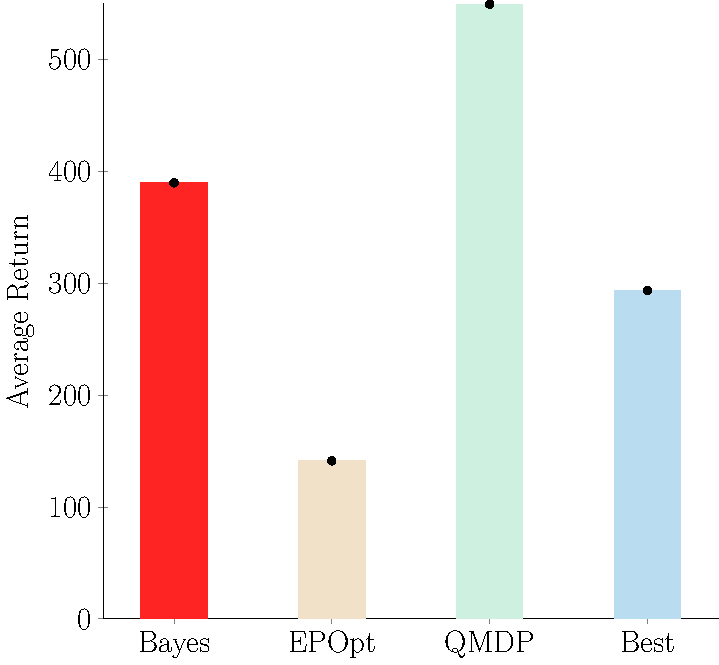
\includegraphics[width=\linewidth]{figs/cheetah_nominal_comparison.pdf}
\subcaption{Nominal MDP}
\label{fig:nominal}
\end{subfigure}
~
\begin{subfigure}[b]{0.3\columnwidth}
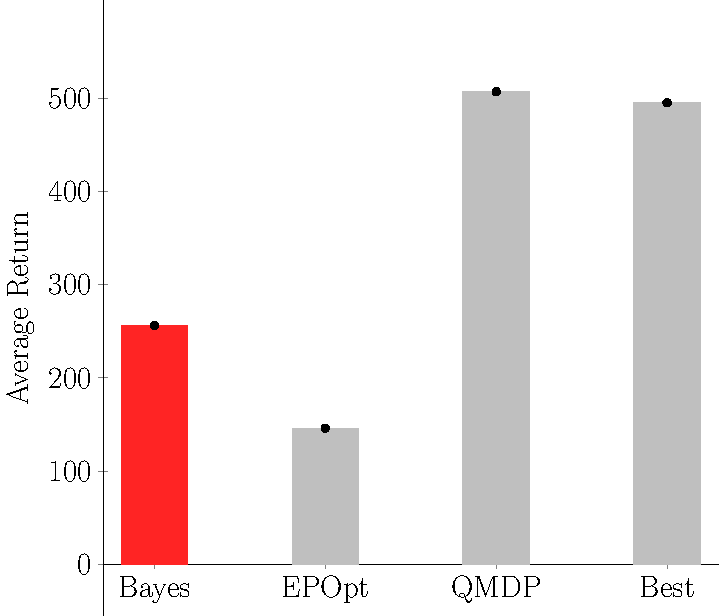
\includegraphics[width=\linewidth]{figs/cheetah_env_comparison.pdf}
\subcaption{One of 20 MDPs}
\label{fig:oneFromK}
\end{subfigure}
~
\begin{subfigure}[b]{0.29\columnwidth}
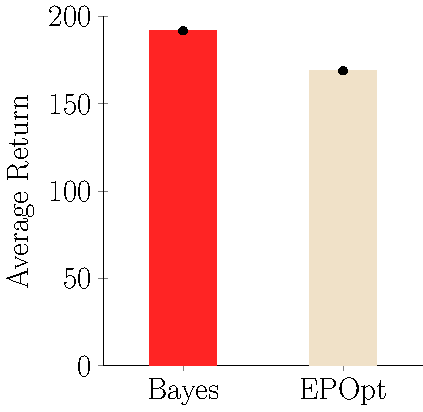
\includegraphics[width=\linewidth]{figs/cheetah_average.pdf}
\subcaption{Over 20 MDPs}
\label{fig:all20}
\end{subfigure}
\end{centering}
\caption{Mean returns on uniformly sampled and prechosen \texttt{HalfCheetah} environments.}
\label{fig:Bars}
\end{figure*}



\section{Conclusion and Future Work}
We presented a policy-gradient algorithm that, by maintaining a belief over latent physical parameters, achieves robustness to model variations and disturbances without compromising significantly on the optimality.
While in this work our belief was over a discrete set of MDPs, there is a natural extension to maintaining a continuous belief distribution either over the MDPs or over the parameter space directly.
A possible extension to enable exploration and distinguish policies (and not just beliefs) is to augment the reward to encourage actions that achieve an information gain.
An immediately interesting avenue worth exploring is to exploit the mixture of experts framework to consider the action proposals from the MDPs along with the belief.


%\begin{itemize}
%    \item Extend to a continuous version which has Gaussian belief distribution as input
%    \item Bootstrap a set of stochastic/deterministic policies, each trained for one MDP or a small range of parameters
%    \item Train with additional reward bonus for information gain which helps distinguishing policies (not just beliefs)
%\end{itemize}


\begin{figure*}[t!]
\begin{centering}
\begin{subfigure}[b]{0.3\columnwidth}
\adjincludegraphics[height=3cm,trim={{.6\width} {0.4\height} {0.15\width} {0.35\height}},clip=true]{figs/keyframes/cheetah/cheetah_nominal.png}
\caption{Nominal}
\end{subfigure}
\begin{subfigure}[b]{0.3\columnwidth}
\adjincludegraphics[height=3cm,trim={{.5\width} {0.4\height} {0.25\width} {0.35\height}},clip=true]{figs/keyframes/cheetah/cheetah_170_92.png}
\caption{Key frames}
\end{subfigure}
\begin{subfigure}[b]{0.3\columnwidth}
\adjincludegraphics[height=3cm,trim={{.5\width} {0.4\height} {0.25\width} {0.35\height}},clip=true]{figs/keyframes/cheetah/cheetah_150_150.png}
\caption{Key frames}
\end{subfigure}
\begin{subfigure}[b]{0.3\columnwidth}
\adjincludegraphics[height=3cm,trim={{.4\width} {0.42\height} {0.35\width} {0.33\height}},clip=true]{figs/keyframes/ant/ant_nominal_18.png}
\caption{Nominal}
\end{subfigure}
\hfill
\begin{subfigure}[b]{0.3\columnwidth}
\adjincludegraphics[height=3cm,trim={{.4\width} {0.42\height} {0.35\width} {0.33\height}},clip=true]{figs/keyframes/ant/ant_120_19.png}
\caption{Key frames}
\end{subfigure}
\hfill
\begin{subfigure}[b]{0.3\columnwidth}
\adjincludegraphics[height=3cm,trim={{.6\width} {0.34\height} {0.15\width} {0.41\height}},clip=true]{figs/keyframes/ant/ant_140_87.png}
\caption{Key frames}
\end{subfigure}
\vfill
\begin{subfigure}[b]{0.3\columnwidth}
\adjincludegraphics[height=3cm,trim={{.55\width} {0.34\height} {0.20\width} {0.41\height}},clip=true]{figs/keyframes/swimmer/swimmer_nominal.png}
\caption{Nominal}
\end{subfigure}
\hfill
\begin{subfigure}[b]{0.3\columnwidth}
\adjincludegraphics[height=3cm,trim={{.55\width} {0.40\height} {0.20\width} {0.35\height}},clip=true]{figs/keyframes/swimmer/swimmer_20_12.png}
\caption{Key frames}
\end{subfigure}
\hfill
\begin{subfigure}[b]{0.3\columnwidth}
\adjincludegraphics[height=3cm,trim={{.35\width} {.2\width} {0.416\width} {0.50\height}},clip=true]{figs/keyframes/swimmer/swimmer_40_157.png}
\caption{Key frames}
\end{subfigure}
\end{centering}
\caption{Keyframes from rollouts on various MDPs. Some of the MDPs are significantly different, so they require drastically different policies to achieve high returns. See \url{https://goo.gl/DN7V9o} for videos.}
\label{fig:frames}
\end{figure*}

\bibliography{intuitive_physics}

\end{document}
